\section{Design}

FlashMatrix is a matrix-oriented programming framework for general data analysis.
This work mainly focuses on dense matrices and scales dense matrix operations
beyond memory capacity by utilizing fast I/O devices, such as solid-state drives
(SSDs), in a non-uniform memory architecture (NUMA).

Figure \ref{fig:arch} shows the architecture of FlashMatrix. The core of
FlashMatrix provides a small number of generalized matrix operators (GenOps)
to simplify the implementation and improve expressiveness of
the framework. The optimizer in FlashMatrix aggressively merges operations to
reduce data movement in the memory hierarchy and achieve better parallelization.
FlashMatrix stores large matrices on SSDs through SAFS \cite{safs},
a user-space filesystem for a large SSD array, to fully utilize high I/O
throughput of SSDs and deploys a set of I/O optimizations to improve
its sequential I/O throughput \cite{SEM_SpMM}.

\begin{figure}
\centering
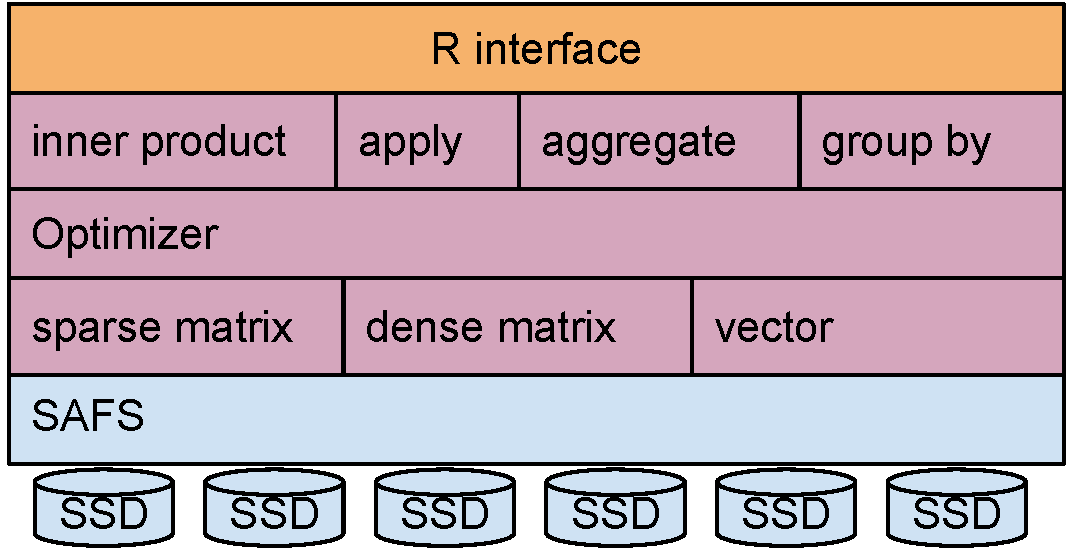
\includegraphics[scale=0.3]{FlashMatrix_figs/architecture.pdf}
\caption{The architecture of FlashMatrix.}
\label{fig:arch}
\end{figure}

\subsection{Programming interface}

FlashMatrix provides a matrix-oriented functional programming interface.
Table \ref{tbl:genops} lists all GenOps, each of which takes matrices and
some functions as input and output new matrices that store computation results.
The input function defines computation on individual elements in input matrices.
The GenOps can be classified into four categories: \textit{apply} for
element-wise operations, \textit{agg} for computing aggregation on a matrix
or on rows/columns of a matrix, \textit{groupby} for splitting rows/columns
of a matrix into multiple groups and computing the aggregation in each group,
\textit{inner product} for computing the inner product of two matrices.

\begin{table}
\begin{center}
\footnotesize
\begin{tabular}{|l|l|l|}
\hline
GenOp & Description \\
\hline
$C=fm.sapply(A, f)$ & $C_{i,j}=f(A_{i,j})$ \\
\hline
$C=fm.mapply(A, B, f)$ & $C_{i,j}=f(A_{i,j}, B_{i,j})$ \\
\hline
$C=fm.mapply.row(A, B, f)$ & $C_{i,j}=f(A_{i,j}, B_j)$ \\
\hline
$C=fm.mapply.col(A, B, f)$ & $C_{i,j}=f(A_{i,j}, B_i)$ \\
\hline
$c=fm.agg(A, f)$ & $c=f(A_{i,j}, c)$, over all $i$, $j$ \\
\hline
$C=fm.agg.row(A, f)$ & $C_i=f(A_{i,j}, C_i)$, over all $j$ \\
\hline
$C=fm.agg.col(A, f)$ & $C_j=f(A_{i,j}, C_j)$, over all $i$ \\
\hline
%$C=fm.groupby(A, f)$ & $C_k=f(A_{i,j}, C_k)$, where $k$ \\
$C=fm.groupby.row(A, B, f)$ & $C_{k,j}=f(A_{i,j}, C_{k,j})$,\\ & where $B_i=k$, over all $i$ \\
\hline
$C=fm.groupby.col(A, B, f)$ & $C_{i,k}=f(A_{i,j}, C_{i,k})$,\\ & where $B_j=k$, over all $j$ \\
\hline
$C=fm.inner.prod(A, B, f1, f2)$ & $t=f1(A_{i,k}, B_{k,j})$,
\\ & $C_{i,j}=f2(t, C_{i,j})$,
\\ & over all $k$ \\
\hline
\end{tabular}
\normalsize
\end{center}
\caption{The list of generalized matrix operators (GenOps) in FlashMatrix.
$A$, $B$ and $C$ are matrices, and $c$ is a scalar.}
\label{tbl:genops}
\end{table}

\begin{comment}
\begin{table}
\begin{center}
\footnotesize
\begin{tabular}{|l|l|l|}
\hline
Class & Function & Description \\
\hline
\multirow{4}{*}{Create} & $fm.rep.int$ & Create a vector of a repeated value \\
& $fm.seq.int$ & Create a vector of sequence numbers \\
& $fm.runif.matrix$ & Create a uniformly random matrix  \\
& $fm.rnorm.matrix$ & Create a random matrix under \\ & & a normal distribution \\
\hline
\multirow{2}{*}{Convert} & $fm.conv.FM2R$ & Convert a FM matrix to an R matrix \\
& $fm.conv.R2FM$ & Convert an R matrix to a FM matrix \\
\hline
\multirow{3}{*}{Reshape} & $t$ & Matrix transpose \\
& $fm.rbind$ & Bind matrices by rows \\
& $fm.cbind$ & Bind matrices by columns \\
\hline
\multirow{4}{*}{Control} & $fm.conv.layout$ & Convert the data layout of a matrix \\
& $fm.set.mate.level$ & Set the materialization level of \\ & & a \textit{virtual matrix} \\
& $fm.materialize$ & Materialize a \textit{virtual matrix} \\
& $fm.conv.store$ & Move a matrix to a specified \\ & & storage \\
\hline
\end{tabular}
\normalsize
\end{center}
\caption{Some of the utility functions in FlashMatrix.}
\label{tbl:utility}
\end{table}

\begin{table}
\begin{center}
\footnotesize
\begin{tabular}{|l|l|l|}
\hline
Class & Function & Description \\
\hline
\multirow{10}{*}{Element-wise} & $C=A+B$ & $C_{i,j}=A_{i,j} + B_{i,j}$ \\
& $C=A-B$ & $C_{i,j}=A_{i,j} - B_{i,j}$ \\
& $C=A*B$ & $C_{i,j}=A_{i,j} * B_{i,j}$ \\
& $C=A/B$ & $C_{i,j}=A_{i,j} / B_{i,j}$ \\
& $C=pmin(A,B)$ & $C_{i,j}=pmin(A_{i,j}, B_{i,j})$ \\
& $C=pmax(A,B)$ & $C_{i,j}=pmax(A_{i,j}, B_{i,j})$ \\
& $C=sqrt(A)$ & $C_{i,j}=sqrt(A_{i,j})$ \\
& $C=abs(A)$ & $C_{i,j}=abs(A_{i,j})$ \\
& $C=exp(A)$ & $C_{i,j}=exp(A_{i,j})$ \\
\hline
\multirow{5}{*}{Aggregate} & $c=sum(A)$ & $c=\sum\limits_{i=1}^{n} \sum\limits_{j=1}^{p}A_{i,j}$ \\
& $C=rowSums(A)$ & $C_i=\sum\limits_{j=1}^{p} A_{i,j}$ \\
& $C=colSums(A)$ & $C_j=\sum\limits_{i=1}^{n} A_{i,j}$ \\
& $c=any(A)$ & true if any element is true \\
& $c=all(A)$ & true if all elements are true \\
\hline
\multirow{1}{*}{multiply} & $\%*\%$ & matrix multiplication \\
\hline
\end{tabular}
\normalsize
\end{center}
\caption{Some of the R functions implemented with GenOps.}
\label{tbl:Rfuns}
\end{table}
\end{comment}

\begin{figure}[t]
\begin{minted}[mathescape,
		fontsize=\scriptsize,
		frame=single,
]{R}
# X is the data matrix
# C is the cluster centers from the previous iteration.
kmeans.iter <- function(X, C)
{
	# Compute the pair-wise distance between a data
	# point and a center.
	D <- fm.inner.prod(X, t(C), "euclidean", "+")
	# Find the closest center to a data point.
	I <- fm.agg.row(D, "which.min")
	# Count the number of data points in each cluster.
	one <- fm.rep.int(1, nrow(I))
	CNT <- fm.groupby.row(one, I, "+")
	# Compute the new centers.
	C <- fm.groupby.row(X, I, "+")
	C <- fm.mapply.row(C, CNT, "/")
	list(C=C, I=I)
}
\end{minted}
\vspace{-5pt}
\caption{The R code of computing an iteration of k-means using GenOps.}
\label{fig:kmeans}
\end{figure}

Figure \ref{fig:kmeans} shows an example of computing an iteration of k-means
\cite{kmeans} using GenOps. It first uses \textit{fm.inner.prod} to
compute the Euclidean distance between every data point and every cluster center,
and outputs a matrix with each row representing the distances from a data
point to every cluster center. It uses \textit{fm.agg.row} to find the closest
cluster for each data point and the output matrix represents how data points
are assigned to clusters. It then uses \textit{fm.groupby.row} to count
the number of data points in each cluster and compute the mean of each cluster.

\subsection{Dense matrices}
Dense matrices are the main data types in FlashMatrix. A vector is stored
as a one-column dense matrix. In FlashMatrix, a dense matrix can be stored
physically in memory or on SSDs or represented virtually by a sequence of
computation. FlashMatrix specifically optimizes for tall-and-skinny matrices
and short-and-wide matrices, and views tall matrices and wide matrices
as groups of tall-and-skinny matrices and short-and-wide matrices, respectively.
In this section, we describe the data format of tall matrices. The similar
strategy is applied to wide matrices.

All matrices in FlashMatrix are immutable and every
matrix operation generates a new matrix. As such, materialization of
\textit{virtual matrices} always generates the same result. FlashMatrix
garbage collects a matrix when there are no references to it.

\subsubsection{Tall-and-skinny matrices} \label{sec:tas_mat}

FlashMatrix optimizes for tall-and-skinny (TAS) dense matrices due to their
frequent occurrence in data analysis. In this field, many data matrices contain
a large number of samples with a relatively few features, so data matrices
are usually tall and skinny. FlashMatrix supports row-major and column-major
matrix layout (Figure \ref{fig:den_mat} (a) and (b)) to avoid data copy for
common matrix operations such as matrix transpose. FlashMatrix optimizes
the generalized matrix operations on TAS dense matrices with tens of columns
or fewer.

\begin{figure}
	\centering
	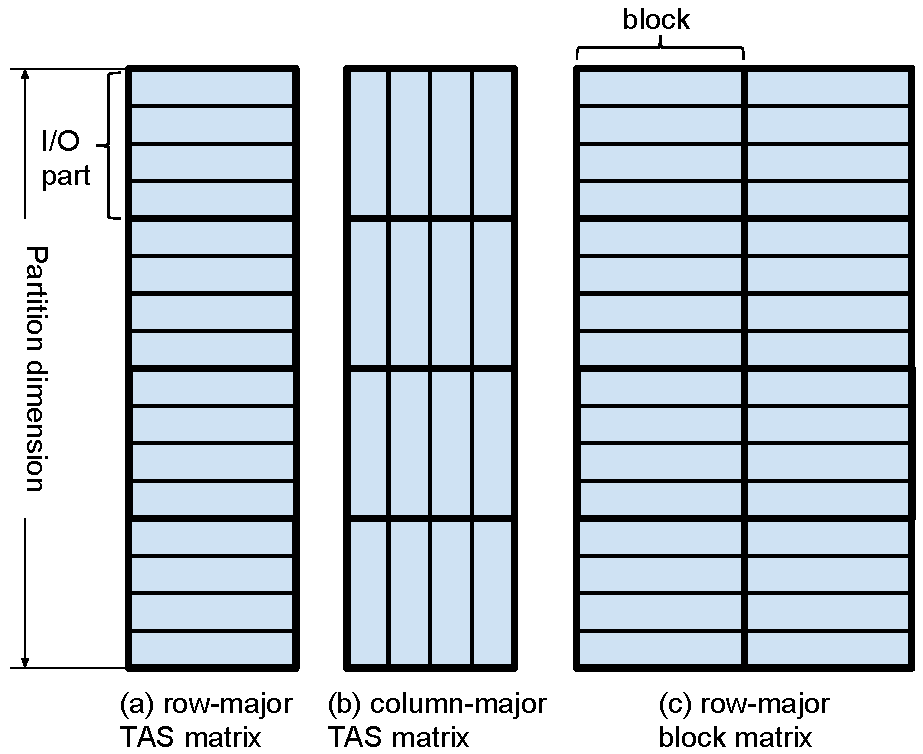
\includegraphics[scale=0.5]{FlashMatrix_figs/dense_matrix2.pdf}
	\caption{The format of a tall dense matrix.}
	\label{fig:den_mat}
\end{figure}

A TAS matrix is partitioned physically into I/O-level partitions (Figure
\ref{fig:den_mat}). All elements in an I/O-level partition are stored
contiguously regardless of the data layout in the matrix. All tall matrices
have the same number of rows in an I/O-level partitions regardless of
the number of columns that the tall matrices have. The number of rows in
an I/O-level partition is always $2^i$. This produces column-major TAS
matrices whose data are well aligned in memory to help CPU vectorization.

\subsubsection{Block matrices} \label{sec:block_mat}
FlashMatrix represents a tall matrix with a group of TAS matrices (Figure
\ref{fig:den_mat} (c)), each with $32$ columns. We refer to such a matrix as
a \textit{block matrix}. To take advantage of the optimizations on matrix
operations on TAS matrices, we decompose a matrix operation on a group of
matrices into operations on individual matrices in the group (Section
\ref{sec:group_op}).
Coupled with the two-level partitioning on TAS matrices, this strategy enables
2D-partitioning on a dense matrix and each partition fits in main memory
or CPU cache.

\subsubsection{Virtual matrices} \label{virt_mat}
In many cases, we do not need to store the data of a matrix physically. Instead,
we compute and generate its data on the fly. Such matrices are essential for
lazy evaluation and we refer to these matrices as \textit{virtual matrices}.
All GenOps may output \textit{virtual matrices} that represent computation
results by storing only the computation of GenOps and the references to input
matrices. \textit{Virtual matrices} are put together to construct a directed
acyclic graph (DAG) to represent a sequence of matrix computation.

%This strategy is essential to reduce data
%movement in the memory hierarchy and memory allocation overhead for creating
%new matrices.

\subsection{Directed acyclic graphs (DAGs)}
The goal is to grow a DAG as large as possible to increase
the ratio of computation and I/O in a DAG. In FlashMatrix, a DAG is a basic
computation task.

\begin{figure}
	\centering
	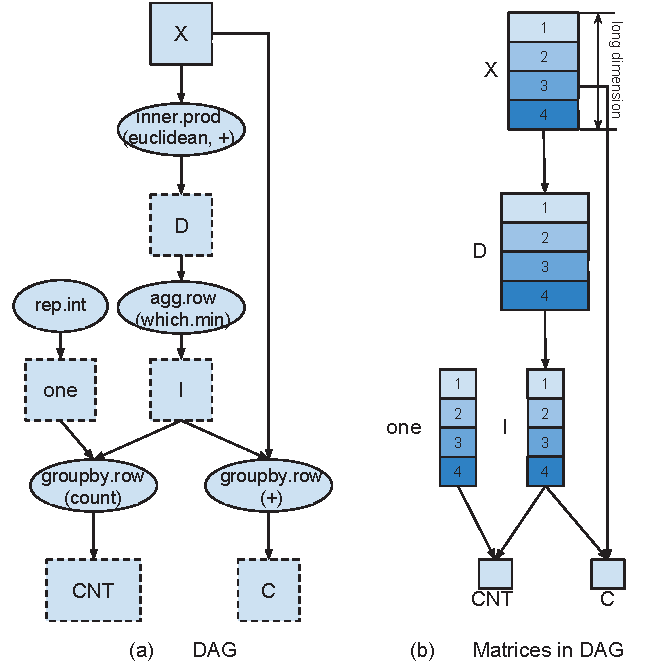
\includegraphics[scale=0.7]{FlashMatrix_figs/KMeans.pdf}
	\caption{A directed acyclic graph of computing an iteration of k-means
	show in Figure \ref{fig:kmeans}.}
	\label{fig:DAG}
\end{figure}

Figure \ref{fig:DAG} (a) shows a DAG for k-means in Figure
\ref{fig:kmeans}. A DAG comprises a set of matrix nodes (shown as rectangles)
and computation nodes (shown as ellipses). Majority of matrix nodes represent
\textit{virtual matrices}, shown as dashed line rectangles, which only contains
the corresponding matrix operations and input matrices. In the case of k-means,
only the input matrix \textit{X} contains materialized data.
A computation node references to a matrix operation and input matrices and
may contain some immutable computation state, such as scalar variables and
small matrices involved in the matrix computation. 

To grow a DAG, FlashMatrix allows \textit{virtual matrices} of different shapes
in a DAG (Figure \ref{fig:DAG} (b)). To simplify evaluation and data flow in
matrix materialization, all \textit{virtual matrices} in the internal matrix
nodes need to have the same \textit{long dimension}. As such, \textit{virtual
matrices} of different sizes in both dimensions form the edge node of a DAG because
any computation that uses these \textit{virtual matrices} cannot be connected
to the same DAG.  We refer to them as \textit{sink matrices}. The GenOps that
generate \textit{sink matrices} are shown in Table \ref{tbl:sink}.

\begin{table}
\begin{center}
\footnotesize
\begin{tabular}{|l|l|l|}
\hline
GenOp & Matrix dim & Output size \\
\hline
fm.agg & ($n \times p$) & $1$ \\
\hline
fm.agg.row & ($n \times p$), $n < p$ & $n$ \\
\hline
fm.agg.col & ($n \times p$), $n > p$ & $p$ \\
\hline
fm.groupby.row & ($n \times p$), $n > p$ & $p \times k$ \\
\hline
fm.groupby.col & ($n \times p$), $n < p$ & $n \times k$ \\
\hline
fm.inner.prod & ($p1 \times n$) $\times$ ($n \times p2$), & $p1 \times p2$ \\
			  & $n \gg p1, n \gg p2$ &  \\
\hline
\end{tabular}
\normalsize
\end{center}
\caption{The GenOps that output \textit{sink matrices}.}
\label{tbl:sink}
\end{table}

\subsection{Materialization of a DAG} \label{sec:materialize}
Access to elements of a \textit{sink matrix} triggers materialization of a DAG.

During materialization of a DAG, FlashMatrix by default saves only the computation
results of sink matrices in the DAG. The computation results are saved in memory
to minimize data written to SSDs. In general, the \textit{sink matrices} shown
in Table \ref{tbl:sink} are small. The maximal size of the output matrix from
an aggregation is $\sqrt{N}$, where $N$ is the number of elements in the input
matrix. The maximal size of the output matrix from a groupby is $k \times \sqrt{N}$,
where $k$ is the number of classes.
For most of machine learning and data analysis tasks, the output matrix of
the inner product of a wide matrix with a tall matrix is usually small because
the long dimension of these matrices is usually much larger than the short
dimension in these tasks.

In some cases, especially in iterative algorithms,
we need to materialize some non-\textit{sink matrices} in a DAG to avoid
redundant computation and I/O across iterations. As such, we allow users to
set a flag on non-\textit{sink matrices} to cache the materialized data in memory
or SSDs during computation, similar to caching a RDD in Spark.

\begin{figure}
	\centering
	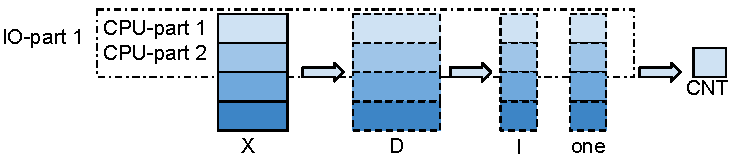
\includegraphics[scale=0.6]{FlashMatrix_figs/materialize.pdf}
	\caption{Materialization of partitions of matrices in a DAG.}
	\label{fig:mater}
\end{figure}

FlashMatrix partitions matrices in a DAG in the \textit{long dimension} and
materializes partitions separately (Figure \ref{fig:mater}). This is realized
because all \textit{virtual matrices} except \textit{sink matrices} in a DAG
share the same \textit{long dimension} size and partition size. As such,
a partition $i$ of a \textit{virtual matrix} only requires data from partitions
$i$ of the parent matrices.
%Owing to
%the storage scheme of in-memory matrices, partitions $i$ of all in-memory
%matrices are stored on the same NUMA node, which minimizes remote memory access.
When materializing a \textit{sink matrix}, each thread first computes partial
aggregation results independently on the partitions of the parent matrix
assigned to the thread. In the end, FlashMatrix merges per-thread partial
aggregation results to construct the \textit{sink matrix}.

FlashMatrix takes advantage of the two-level partitioning on dense matrices
to reduce data movement between SSDs and CPU. It assigns I/O-level partitions
to a thread as computation tasks for parallelization. We choose a relatively
small partition size to balance the overhead of accessing a partition,
computation skew and memory consumption. A thread further splits
an I/O-level partition into CPU-level partitions at run time and materializes
one CPU-level partition at a time. Materialization of a CPU-level partition
is triggered recursively. As shown in Figure \ref{fig:mater}, materializing
matrix \textit{CNT} triggers materialization of CPU-level partitions of matrices
\textit{I} and \textit{one}, which in turn triggers materialization of
partitions of matrix \textit{D}, and so on. Eventually, it triggers data access
to an I/O-level partition of input matrix \textit{X} from SSDs.
After materializing a CPU-level partition, the thread passes it to the subsequent
operation, instead of materializing the next CPU-level partition in the same matrix.
A CPU-level partition is sufficiently small to fit in the CPU cache so that
the partition still resides in the CPU cache when the subsequent operation consumes
it. This significantly reduces data movement between CPU and memory. In each
thread, all intermediate matrices have only one CPU-level partitions materialized
at any time to reduce CPU cache pollution and thus increase CPU cache hits.
%To reduce CPU cache polution, a CPU-level partition is discarded once it is
%used by all children matrices.

%In a DAG, a matrix may be
%required by multiple GenOps. As such, each matrix always buffers one materialized
%CPU-level partition in each thread to avoid redundant computation.

% TODO
%To keep data in CPU cache as long as possible, we reuse the memory buffers
%to reduce the number of memory buffers used in the computation and avoid CPU
%cache polution.

\subsection{Parallel execution and I/O access}
When materializing a DAG in parallel, FlashMatrix dispatches computation tasks
in such a way that we issue large reads and merge writes to SSDs while still
achieving good load balancing.

FlashMatrix uses a global task scheduler to assign tasks that contain
computation on I/O-level partitions to threads dynamically. At the beginning,
the task scheduler assigns multiple contiguous I/O-level partitions to a thread
so that the thread can read these I/O-level partitions from a matrix with
a single I/O. As the computation in a DAG approaches to an end, the scheduler
dispatches tasks with a single I/O-level partitions. The task scheduler also
ensures that all threads work on I/O-level partitions that are adjacent to
each other. As such, if materialization of a DAG requires to storing the materialized
result of a non-\textit{sink matrix}, the execution order helps us to merge
writes from multiple threads to achieve sustainable write throughout and reduce
write amplification \cite{}.

%For a block matrix with many TAS matrices, we parallelize the computation and
%I/O access differently. One of the goals is to reduce memory consumption.
%Instead of getting the row/column range from all TAS matrices before performing
%computation, we read the row/column range from some TAS matrices first, perform
%computation and move on to the next TAS matrices in the same range. This is
%very helpful if the computation is aggregation.
